\section{Learning a default strategy}
\label{sec:part2}
In the previous chapter we created a calculator that can determine the strength of a hand by calculating the probability of winning. In this chapter we shall use the calculator to calculate the strength of the hands.\\

When the APC first joins a poker game it has no information about the opponent, and in this case it must use a default strategy while it gathers more information.

In this chapter we will find a solution to the problem statement:

\vspace{4mm}
\begin{statementBox2}{Problem statement 2}
How can one develop a default strategy without having information about the opponents?
\end{statementBox2}
\vspace{4mm}

Even though players have different strategies they often have some decisions in common. Most players tend to play more aggressively the better their chances are of winning and likewise most players will fold if they have a weak hand. These tendencies can be used in a default strategy. The popular decisions are more likely to be good. For instance, most players agree that it is unwise to fold a pair of aces in the pre-flop. 

The default strategy has to work against every strategy, therefore it is impossible for it to be better than all of them. The goal for the default strategy is not to win, although that is preferable, but instead to reduce the loses while it gathers information about the opponent.

\subsection{Design}
To develop a strategy in poker the two most commonly used options are to either directly program the procedures in the code or to create a self-learning algorithm. 

Programming the procedures in the code requires the programmer to have a deep insight in how to play poker and how to make the optimal decisions during a game. One can also use the expertise of professional poker players in case one lacks the insight.

The self-learning algorithm uses the concept watch and learn by observing other players and trying to learn the strategy behind their decisions. This method requires that the algorithm has someone to observe.

Since we do not have any particular insight in how to play poker and do not have expertise from any professional poker players, we will implement a self-learning algorithm. Additionally, by using this method the computer is not limited by our understanding of the game. We will use data from real life poker games for the algorithm. The data is further described in section \ref{sec:default-test}.\\

To implement the self-learning algorithm we use an artificial neural network (ANN), see section \ref{sec:nn}. The ANN is well suited for finding patterns of the players decisions. 

Our goal is to design an ANN with a total network error (TNE) of five percent or less. We find five percent to be acceptable as players often take irrational decisions and the ANN only tries to find an approximation of the results. 

We use an iterative development method to design the ANN. We start by designing a simple ANN and then move on to more complex ANN's.\\

All our ANN's have exactly two outputs. The first output is whether or not to be defensive by checking or calling and the second output is whether or not to be aggressive by betting or raising. The closer an output is to the value one, the more certain the ANN is, that it is the correct decision. 

All our ANN's use normalised inputs and a sigmoid function as transfer function. The reason we settle for a sigmoid function rather than a step function is because the sigmoid function allows us to see how certain the ANN is of each decision being correct.

\subsubsection{Artificial neural network (ANN)}
\label{sec:nn}
An artificial neural network (ANN) is inspired by the human brain. It can be used for pattern recognition or classification among other things. An ANN can take any number of inputs and return any number of outputs. 

An ANN is made up of neurons that are connected into a network. Each neuron takes a set of inputs and returns a single output. The output of a neuron is sent to all the connected neurons. Each input has a weight that determines influence of the input. The neuron uses an input function to calculate the net input, usually the sum of all weighted inputs, and pass it on to the transfer function. The type of transfer function determines the output. A step function returns zero or one if the net input is above a certain threshold. This is useful for logical functions. If one needs a value between zero and one a sigmoidal function can be used instead.

Figure \ref{fig:neuron} models a neuron. Here the weighted inputs $w_{i1}$, $w_{i2}$, and $w_{i3}$ are all send to the input function $\sum$ which then calculates the net input $net_{i}$. The transfer function $f$ then calculates the output from the net input.

\begin{figure}[H]
  \center
    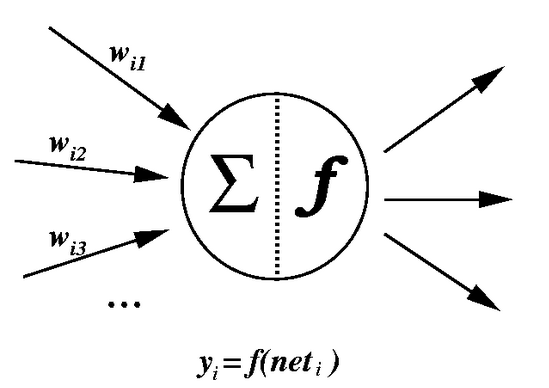
\includegraphics[scale=0.4]{images/nn/neuron.png}
  \caption{Model of a neuron.\cite{neuron} \label{fig:neuron}}
\end{figure}

The neurons in an ANN are distributed in layers as shown in figure \ref{fig:perceptron} and \ref{fig:mlp}. The coloured circles represents neurons and the arrows represents the connections between the neurons. There are three layers, an input layer, a hidden layer, and an output layer. An ANN consists of one input layer and one output layer but may contain any number of hidden layers. The simplest type of ANN is the perceptron which has no hidden layers, see figure \ref{fig:perceptron}. It is used for single calculations. A multilayer perceptron is another type of ANN which contains hidden layers. It is used for more complex domains with multiple layers of computations. 

\def\layersep{2.5cm}

\begin{figure}[H]
\center
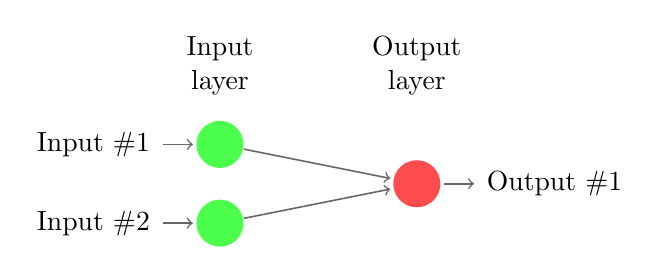
\begin{tikzpicture}[shorten >=1pt,->,line width=0.2mm,draw=black!60, node distance=\layersep]
    \tikzstyle{every pin edge}=[<-,shorten <=1pt]
    \tikzstyle{neuron}=[circle,fill=black!25,minimum size=17pt,inner sep=0pt]
    \tikzstyle{input neuron}=[neuron, fill=green!70];
    \tikzstyle{output neuron}=[neuron, fill=red!70];
    \tikzstyle{hidden neuron}=[neuron, fill=blue!70];
    \tikzstyle{annot} = [text width=4em, text centered]

    % Draw the input layer nodes
    \node[input neuron, pin=left:Input \#1] (I-1) at (0,-1) {};
    \node[input neuron, pin=left:Input \#2] (I-2) at (0,-2) {};

    % Draw the output layer node
    \node[output neuron,pin={[pin edge={->}]right:Output \#1}] (O-1) at (\layersep,-1.5) {};

    % Connect every node in the input layer with every node in the
    % hidden layer.
    \path (I-1) edge (O-1);
    \path (I-2) edge (O-1);

    % Annotate the layers
    \node[annot,above of=I-1, node distance=1cm] (il) {Input layer};
    \node[annot,right of=il] {Output layer};
\end{tikzpicture}
\caption{Perceptron with two inputs and one output. \label{fig:perceptron}}
\end{figure}
\vspace{4mm}
\def\layersep{2.5cm}

\begin{figure}[H]
\center
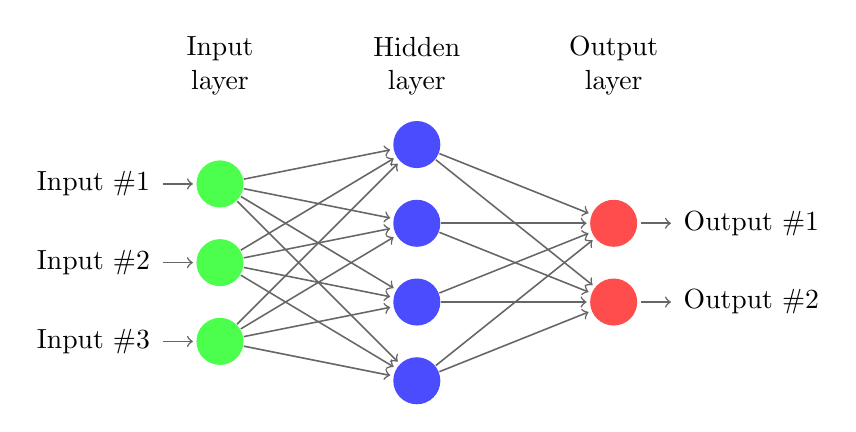
\begin{tikzpicture}[shorten >=1pt,->,line width=0.2mm,draw=black!60, node distance=\layersep]
    \tikzstyle{every pin edge}=[<-,shorten <=1pt]
    \tikzstyle{neuron}=[circle,fill=black!25,minimum size=17pt,inner sep=0pt]
    \tikzstyle{input neuron}=[neuron, fill=green!70];
    \tikzstyle{output neuron}=[neuron, fill=red!70];
    \tikzstyle{hidden neuron}=[neuron, fill=blue!70];
    \tikzstyle{annot} = [text width=4em, text centered]

    % Draw the input layer nodes
    %\foreach \name / \y in {1,...,4}
    % This is the same as writing \foreach \name / \y in {1/1,2/2,3/3,4/4}
    \node[input neuron, pin=left:Input \#1] (I-1) at (0,-1.5) {};
    \node[input neuron, pin=left:Input \#2] (I-2) at (0,-2.5) {};
    \node[input neuron, pin=left:Input \#3] (I-3) at (0,-3.5) {};

    % Draw the hidden layer 1 nodes
    \node[hidden neuron] (H-1) at (\layersep,-1) {};
    \node[hidden neuron] (H-2) at (\layersep,-2) {};
    \node[hidden neuron] (H-3) at (\layersep,-3) {};
    \node[hidden neuron] (H-4) at (\layersep,-4) {};

    % Draw the output layer node
    \node[output neuron,pin={[pin edge={->}]right:Output \#1}] (O-1) at (2*\layersep,-2) {};
    \node[output neuron,pin={[pin edge={->}]right:Output \#2}] (O-2) at (2*\layersep,-3) {};

    % Connect every node in the input layer with every node in the
    % hidden layer.
    \path (I-1) edge (H-1);
    \path (I-2) edge (H-1);
    \path (I-3) edge (H-1);
    \path (I-1) edge (H-2);
    \path (I-2) edge (H-2);
    \path (I-3) edge (H-2);
    \path (I-1) edge (H-3);
    \path (I-2) edge (H-3);
    \path (I-3) edge (H-3);
    \path (I-1) edge (H-4);
    \path (I-2) edge (H-4);
    \path (I-3) edge (H-4);
    
    % Connect every node in the hidden layer with the output layer
    \path (H-1) edge (O-1);
    \path (H-1) edge (O-2);
    \path (H-2) edge (O-1);
    \path (H-2) edge (O-2);
    \path (H-3) edge (O-1);
    \path (H-3) edge (O-2);
    \path (H-4) edge (O-1);
    \path (H-4) edge (O-2);

    % Annotate the layers
    \node[annot,above of=H-1, node distance=1cm] (hl) {Hidden layer};
    \node[annot,left of=hl] {Input layer};
    \node[annot,right of=hl] {Output layer};
\end{tikzpicture}
\caption{Multilayer perceptron with three inputs and two outputs. \label{fig:mlp}}
\end{figure}

The ANN can be trained using a training set of inputs. Using supervised learning, in contrast to unsupervised learning, one must also supply an expected output. For each input it will adjust the weights in order to get closer to the expected output. The TNE indicates the amount of training data that did not produce the expected result. The TNE is calculated during each iteration and the ANN will continue adjusting the weights until the TNE is acceptable. 

Backpropagation is the most common algorithm for supervised ANNs. It adjust the weights from the end (the output neurons) back to the start (the input neurons).

After the training the ANN can be validated to see if it works. This is done using a test set different from the training set and see if the results of the ANN matches the expected results of the test set.

\subsubsection{First ANN design}
\label{sec:design1}
For the first attempt we design a simple perceptron that takes two inputs, and returns two outputs, see figure \ref{fig:nn1}. 
\def\layersep{2.5cm}

\begin{figure}[H]
\center
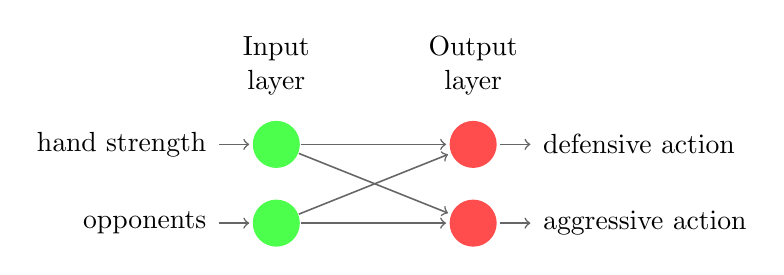
\begin{tikzpicture}[shorten >=1pt,->,line width=0.2mm,draw=black!60, node distance=\layersep]
    \tikzstyle{every pin edge}=[<-,shorten <=1pt]
    \tikzstyle{neuron}=[circle,fill=black!25,minimum size=17pt,inner sep=0pt]
    \tikzstyle{input neuron}=[neuron, fill=green!70];
    \tikzstyle{output neuron}=[neuron, fill=red!70];
    \tikzstyle{hidden neuron}=[neuron, fill=blue!70];
    \tikzstyle{annot} = [text width=4em, text centered]

    % Draw the input layer nodes
    \node[input neuron, pin=left:hand strength] (I-1) at (0,-1) {};
    \node[input neuron, pin=left:opponents] (I-2) at (0,-2) {};

    % Draw the output layer node
    \node[output neuron,pin={[pin edge={->}]right:defensive action}] (O-1) at (\layersep,-1) {};
    \node[output neuron,pin={[pin edge={->}]right:aggressive action}] (O-2) at (\layersep,-2) {};

    % Connect every node in the input layer with every node in the
    % hidden layer.
    \path (I-1) edge (O-1);
    \path (I-2) edge (O-1);
    \path (I-1) edge (O-2);
    \path (I-2) edge (O-2);

    % Annotate the layers
    \node[annot,above of=I-1, node distance=1cm] (il) {Input layer};
    \node[annot,right of=il] {Output layer};
\end{tikzpicture}
\caption{First ANN design. \label{fig:nn1}}
\end{figure}

The first input is the hand strength. We use the calculator from chapter \ref{sec:part1} to calculate the probability of winning against a single opponent. The reason we always find the probability against a single opponent is because the probability of winning decreases drastically as the number of opponents increases. We use an absolute hand strength rather than a hand strength relative to the number of players. This makes it easier to compare the hands strengths in situations with different numbers of players. 

The second input is the number of opponents. The input is normalized as \[I_{norm} = \frac{Opp}{Opp_{max}}\] 
Here $Opp$ is the number of opponents and $Opp_{max}$ is the maximum number of opponents (in our case nine).

From the tests we found that this network had a TNE of $\sim$19,9 \%, see section \ref{sec:ann-test1}. This does not fulfil our requirement of a TNE of five percent or less.

\subsubsection{Second ANN design}
Since the first approach designing a perceptron did not fulfil our requirement we instead design a multilayer perceptron (MLP) with five inputs.

The MLP is taking the same inputs as the perceptron from section \ref{sec:design1}, but now it takes three additional inputs: The chips of the player, the cost for the player to call, and the pot. We normalize the three new inputs as: \[I_{norm} = \frac{I}{chips_{total}}\]. 
Here $I$ is the input to be normalized and $chips_{total}$ is the total amount of chips in the game, including the pot and the bets.

The MLP has one hidden layer with two hidden neurons. One hidden neuron to calculate the likelihood of winning and another for the economically aspect.

\def\layersep{2.5cm}

\begin{figure}[H]
\center
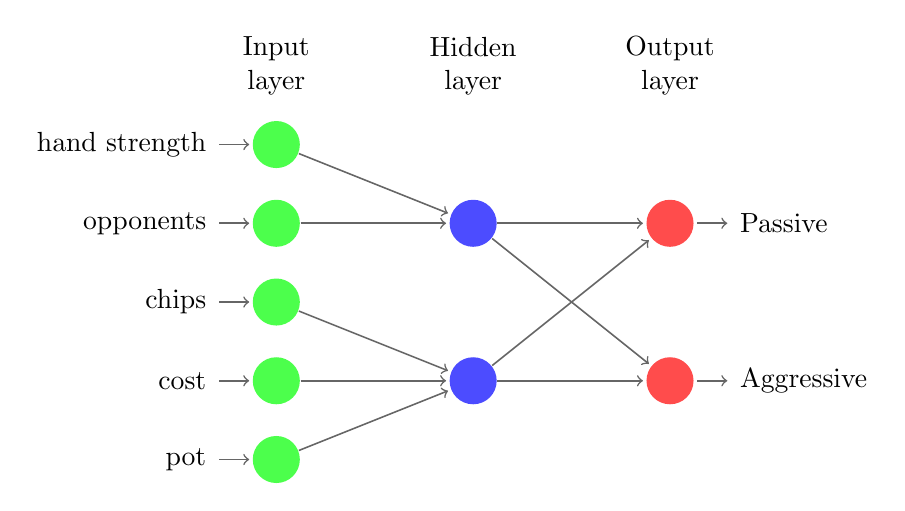
\begin{tikzpicture}[shorten >=1pt,->,line width=0.2mm,draw=black!60, node distance=\layersep]
    \tikzstyle{every pin edge}=[<-,shorten <=1pt]
    \tikzstyle{neuron}=[circle,fill=black!25,minimum size=17pt,inner sep=0pt]
    \tikzstyle{input neuron}=[neuron, fill=green!70];
    \tikzstyle{output neuron}=[neuron, fill=red!70];
    \tikzstyle{hidden neuron}=[neuron, fill=blue!70];
    \tikzstyle{annot} = [text width=4em, text centered]

    % Draw the input layer nodes
    %\foreach \name / \y in {1,...,4}
    % This is the same as writing \foreach \name / \y in {1/1,2/2,3/3,4/4}
    \node[input neuron, pin=left:hand strength] (I-1) at (0,-1) {};
    \node[input neuron, pin=left:opponents] (I-2) at (0,-2) {};
    \node[input neuron, pin=left:chips] (I-3) at (0,-3) {};
    \node[input neuron, pin=left:cost] (I-4) at (0,-4) {};
    \node[input neuron, pin=left:pot] (I-5) at (0,-5) {};

    % Draw the hidden layer nodes
    \node[hidden neuron] (H-1) at (\layersep,-2) {};
    \node[hidden neuron] (H-2) at (\layersep,-4) {};

    % Draw the output layer node
    \node[output neuron,pin={[pin edge={->}]right:Passive}] (O-1) at (2*\layersep,-2) {};
    \node[output neuron,pin={[pin edge={->}]right:Aggressive}] (O-2) at (2*\layersep,-4) {};

    % Connect every node in the input layer with every node in the
    % hidden layer.
    \path (I-1) edge (H-1);
    \path (I-2) edge (H-1);
    \path (I-3) edge (H-2);
    \path (I-4) edge (H-2);
    \path (I-5) edge (H-2);
    
    % Connect every node in the hidden layer with the output layer
    \path (H-1) edge (O-1);
    \path (H-1) edge (O-2);
    \path (H-2) edge (O-1);
    \path (H-2) edge (O-2);

    % Annotate the layers
    \node[annot,above of=I-1, node distance=1cm] (il) {Input layer};
    \node[annot,right of=il] (hl) {Hidden layer};
    \node[annot,right of=hl] {Output layer};
\end{tikzpicture}
\caption{Second ANN design. \label{fig:nn2}}
\end{figure}

Vi har ikke nået mere så du behøver ikke læse videre :)

\subsection{Test}
\label{sec:default-test}

The University of Alberta has a research group that specializes in the field of artificial intelligence in poker \cite{alberta}. They have released a dataset containing data from $\sim$18.000 real-life rounds of Texas hold'em limit poker. The dataset only contains data about the hole cards of the players who made it to the showdown. We will refer to these players as relevant players.

The dataset consists of multiple files. The file called \textit{hroster} contains the names of all players at the beginning of the round. The file called \textit{hdb} contains the information about the community cards and the flop after each game state. For each player a file called \textit{pdb.}<playername> exists. This file includes the hole cards (if the player did not fold), chips, profit from round and actions during each game state. 

We have collected all the data from the different files into an single file called \textit{refactored-data.txt} to make it easier analyse the rounds. We discarded the data for all rounds that has no relevant players. This is because no information about the hole cards exists in such rounds and therefore it is irrelevant for us. 

This dataset will be used for training and testing the ANN's throughout this section.\\

To create and test the ANN's we use a framework called Neuroph cite{neuroph}. Neuroph is a neural network framework programmed in java. 

\subsubsection{Find the TNE of the first ANN}
\label{sec:ann-test1}
We create a dataset containing the information about the game for each action performed by a relevant player. All informations about the game is found for the moment of the action. For instance, an action in the pre-flop will have no information about the community cards.
The dataset contains data from $\sim$1300 actions distributed across all game states.

For this test the dataset only includes the hole cards of the player, the community cards and the number of opponents.

To find the TNE of the perceptron described in section \ref{sec:design1}, we train it using our dataset. The graph seen in figure \ref{fig:tneg1} displays the TNE through each iteration of the training. From the graph we can see that the TNE does not get any smaller than $\sim$19,9 \%.

\begin{figure}[H]
  \center
    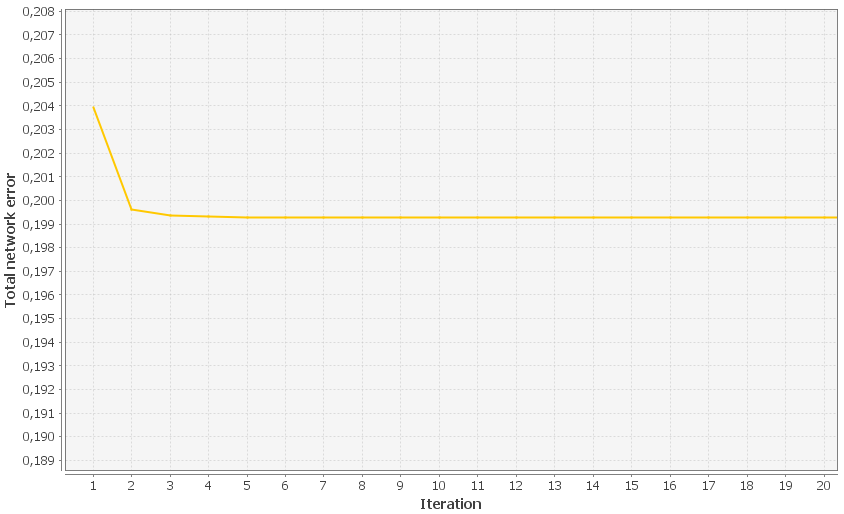
\includegraphics[scale=0.6]{images/nn/default-nn1-err.png}
  \caption{TNE graph from training the first ANN.\label{fig:tneg1}}
\end{figure}

To see 

\subsubsection{Find the TNE of the second ANN}
\label{sec:ann-test2}
some text

\subsection{Discussion}
When artificial intelligence starts out by playing the games of poker it doesn't have any kind of information about the opponents. So to make sure that the bot wont just go keep throwing away the bank roll. Instead we wanted the bot to minimizes our losses so that we would still have a decent bank roll when we have gathered information about the opponents so that the bot could make qualified guesses at what move would be the most appropriate in terms of the current opponent. The default player was never meant to be on the same level as a human player, but humans are only in a slightly better position than the default bot. The human player can like the bot only see the hole and community cards, but a human is also able to make a profile of the bot in their head. This means that they can learn how the bot decides and exploit this. 
This is one of the reasons that we chose to go with a neural network. In a neural network we are able to of course train the network to make correct decisions based on the targeted output that we give it.
But as the game proceeds the neural network has an input which will weight when we have enough information about the opponents to shift our gameplay from the default play style to a more adaptive one.
The time that it takes a human player to learn about the bot and adapt to it, should be the same for the bot. So if we imagine a human player who is good enough to decipher the way the bot is playing and adapt to it. When the human player does that, the bot should also have started to change its ways. Slowly as the bot learn it will adapt more and more to the opponent so when we have enough information the bot will shift completely and disregard the default play style.
\subsection{Conclusion}
